\newpage
\section{Auswertung}
%Schonmal die Tabellen für dich ;-)


%data2


%data3
\begin{table}
    \centering
    \begin{tabular}{c c c}
        \toprule
        $I_{Spule} \;/\;$A & $U_H\;/\;$mV & $I_{durch} \;/\;$A\\
        \midrule
        0                   &0,0081              &10\\
        0,5                 &0,0055              &10\\
        1,0                 &0,0039              &10\\
        1,5                 &0,0012              &10\\
        2,0                 &-0,0008             &10\\
        2,5                 &-0,0025             &10\\
        3,0                 &-0,0048             &10\\
        3,5                 &-0,0068             &10\\
        4,0                 &-0,0086             &10\\
        4,5                 &-0,0097             &10\\
        5,0                 &-0,0110             &10\\
        \bottomrule
    \end{tabular}
    \caption{Hall Spannung für Kupfer- konstanter Duchflussstrom}
    \label{tab:Cu_B}
\end{table}

%data4


%data5


%data6
\begin{table}
    \centering
    \begin{tabular}{c c c}
        \toprule
        $I_{Spule} \;/\;$A & $U_H\;/\;$mV & $I_{durch} \;/\;$A\\
        \midrule
            5                   &-0,0012&             0\\
            5                   &-0,0373&             1\\
            5                   &-0,0755&             2\\
            5                   &-0,1136&             3\\
            5                   &-0,1530&             4\\
            5                   &-0,1919&             5\\
            5                   &-0,2291&             6\\
            5                   &-0,2671&             7\\
            5                   &-0,3090&             8\\
            5                   &-0,3512&             9\\
            5                   &-0,3957&             10\\
        \bottomrule
    \end{tabular}
    \caption{Hall Spannung für Zink- konstantes Magnetfeld}
    \label{tab:Zn_B}
\end{table}

%data7
\begin{table}
    \centering
    \begin{tabular}{c c c}
        \toprule
        $I_{Spule} \;/\;$A & $U_H\;/\;$mV & $I_{durch} \;/\;$A\\
        \midrule
            0                   &-0,1707&             10\\
            0,5                 &-0,1740&             10\\
            1,0                 &-0,1777&             10\\
            1,5                 &-0,1809&             10\\
            2,0                 &-0,1850&             10\\
            2,5                 &-0,1885&             10\\
            3,0                 &-0,1909&             10\\
            3,5                 &-0,1945&             10\\
            4,0                 &-0,1970&             10\\
            4,5                 &-0,1990&             10\\
            5,0                 &-0,2002&             10\\
       \bottomrule
    \end{tabular}
    \caption{Hall Spannung für Silber- konstanter Durchflussstrom}
    \label{tab:Ag_I}
\end{table}

%data8
\begin{table}
    \centering
    \begin{tabular}{c c c}
        \toprule
        $I_{Spule} \;/\;$A & $U_H\;/\;$mV & $I_{durch} \;/\;$A\\
        \midrule
  5                   &0,0005&              0\\
  5                   &-0,0207&             1\\
  5                   &-0,0394&             2\\
  5                   &-0,0599&             3\\
  5                   &-0,0794&             4\\
  5                   &-0,0991&             5\\
  5                   &-0,1185&             6\\
  5                   &-0,1394&             7\\
  5                   &-0,1602&             8\\
  5                   &-0,1821&             9\\
  5                   &-0,2026&             10\\

       \bottomrule
    \end{tabular}
    \caption{Hall Spannung für Silber- konstantes Magnetfeld}
    \label{tab:Ag_I}
\end{table}
\subsection{Magnetfeldmessung}
Zu Beginn des Experiments wird das Magnetfeld in Abhängigkeit des Spulenstroms bestimmt (\ref{tab:Br}).
Zwischen den beiden Größen besteht ein linearer Zusammenhang, daher lässt sich die Kurve durch eine Ausgleichsgerade annähern.
% Data 2
\begin{table}[H]
    \centering
    \begin{tabular}{c c}
        \toprule
        $I_{Spule} \;/\;$A & $B\;/\;$mT\\
        \midrule
        0,0                 &0,0\\
        0,5                 &132,4\\
        1,0                 &270,0\\
        1,5                 &413,7\\
        2,0                 &556,4\\  
        2,5                 &698,3\\
        3,0                 &828,3\\
        3,5                 &956,0\\
        4,0                 &1063,9\\
        4,5                 &1145,2\\
        5,0                 &1204,5\\
        \bottomrule
    \end{tabular}
    \caption{Magnetfeldmessung (reihe)}
    \label{tab:Br}
\end{table}
% Plot 2
\begin{figure}[H]
    \centering
    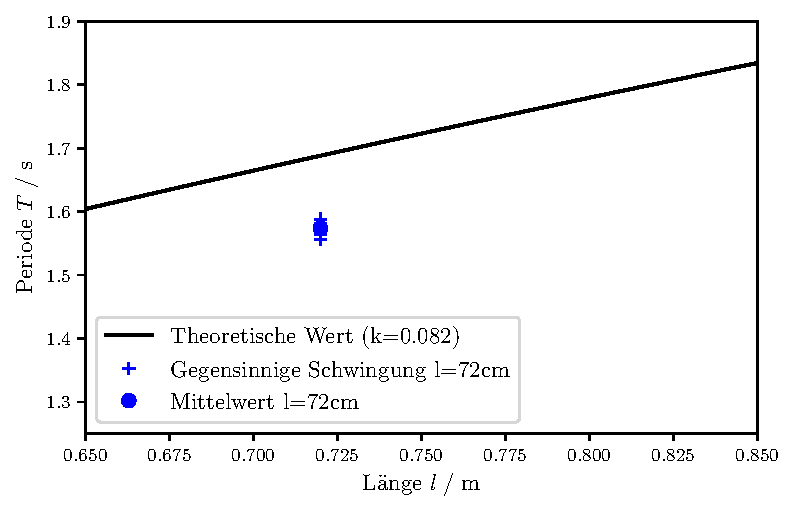
\includegraphics{build/plot2.pdf}
    \caption{B-Feld Messung}
    \label{fig:Br}
\end{figure}
Mit der Ausgleichsgeraden
\begin{align*}
    y &= mx + b\\
    m &= 251\pm 8\\  
    b &= 32\pm 24\\
\end{align*}
Aus der Umkerfunktion dieser Ausgleichsrechnung lässt sich in den folgenden Berechnungen das B-Feld aus dem angelegten Spulenstrom bestimmen.
% --------KUPFER
\subsection{Kupfer}
\subsubsection{Geometrische Messungen und Wiederstand}
Die Dicke des Kupferblatts konnte auf der Apparatur abgelesen werden.
Die Länge des Kupferdrahts konnte auch abgelesen werden, der Wiederstand wurde jedoch gemessen.
\begin{align*}
    d_{Cu} &= \SI{18}{\micro \meter} \\
    l_{Cu} &= \SI{137}{\centi \meter}\\
    R_{Cu} &= \SI{2,734}{\ohm}\\
    r_{Cu} &= \frac{1}{2}\cdot \SI{0,218}{\milli \meter}
\end{align*}
Daraus lässt sich die spezifische Leitfähigkeit des Materials berechnen.
\begin{align*}
    \rho_{Cu} &= R_{Cu}\cdot \frac{\pi r_{Cu}^2}{l_{Cu}}\\
    rho_{Cu} &= \SI{0,074\pm0,007}{\micro \ohm \meter}\\
    \rho_{Cu,literatur} &= \SI{0,018}{\micro \ohm \meter} %https://oerttel.net/data/documents/Leitfaehigkeit.pdf
\end{align*}
Ab hier wird mit dem Literaturwert weitergerechnet(Erklärung: \ref{sec:Diskussion}).
\subsubsection{Hall Spannung bei konstantem B-Feld}
Um die Abhängigkeit der Hall Spannung vom anliegenden Querstrom $I_q$ festzustellen wurde der Spulenstrom $I_B$ konstant auf 5 Ampere gehalten.
% Data 4
\begin{table}[H]
    \centering
    \begin{tabular}{c c c}
        \toprule
        $I_B \;/\;$A & $U_H\;/\;$mV & $I_q \;/\;$A\\
        \midrule
            5                   & 0,0029&             0\\
            5                   & 0,0005&             1\\
            5                   &-0,0015&             2\\
            5                   &-0,0030&             3\\
            5                   &-0,0044&             4\\
            5                   &-0,0056&             5\\
            5                   &-0,0075&             6\\
            5                   &-0,0088&             7\\
            5                   &-0,0110&             8\\
            5                   &-0,0129&             9\\
            5                   &-0,0140&             10\\
        \bottomrule
    \end{tabular}
    \caption{Hall Spannung für Kupfer- konstantes Magnetfeld}
    \label{tab:Cu_I}
\end{table}
% Plot 4
\begin{figure}[H]
    \centering
    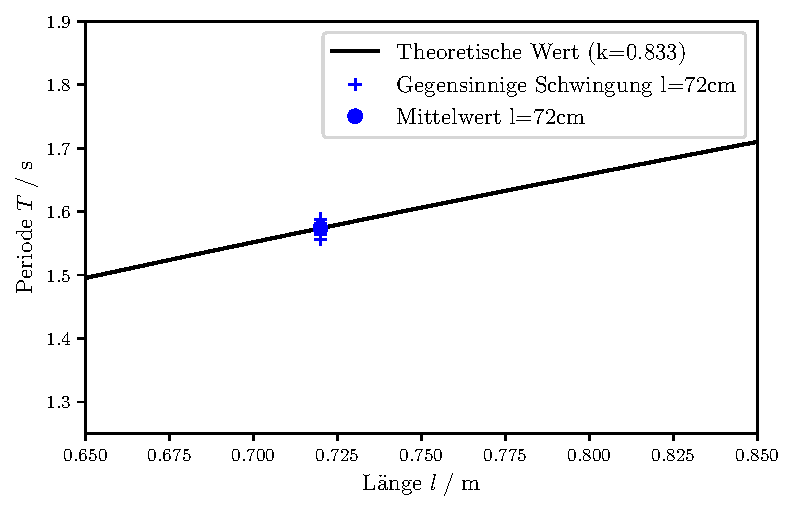
\includegraphics{build/plot4.pdf}
    \caption{Hall Spannung in Abhängigkeit vom Querstrom - Kupfer}
    \label{fig:Cu_I}
\end{figure}
Mit der Ausgleichsgeraden
\begin{align*}
    y &= mx + b\\
    m &= -0.001654\pm 0.00004\\  
    b &=  0.0023\pm 0.0003\\
\end{align*}

\subsubsection{Hall Spannung bei konstantem Querstrom}
Um die Abhängigkeit der Hall Spannung vom äußeren Magnetfeld $B$ festzustellen wurde der Querstrom $I_q$ konstant auf 10 Ampere gehalten.
% Data 5
\begin{table}
    \centering
    \begin{tabular}{c c c}
        \toprule
        $I_{Spule} \;/\;$A & $U_H\;/\;$mV & $I_{durch} \;/\;$A\\
        \midrule
            0                   &-0,4094&             10\\
            0,5                 &-0,4042&             10\\
            1,0                 &-0,4024&             10\\
            1,5                 &-0,4004&             10\\
            2,0                 &-0,3981&             10\\
            2,5                 &-0,3981&             10\\
            3,0                 &-0,3950&             10\\
            3,5                 &-0,3928&             10\\
            4,0                 &-0,3900&             10\\
            4,5                 &-0,3880&             10\\
            5,0                 &-0,3800&             10\\
        \bottomrule
    \end{tabular}
    \caption{Hall Spannung für Zink- konstanter Durchflussstrom}
    \label{tab:Zn_I}
\end{table}
% Plot 5
\begin{figure}[H]
    \centering
    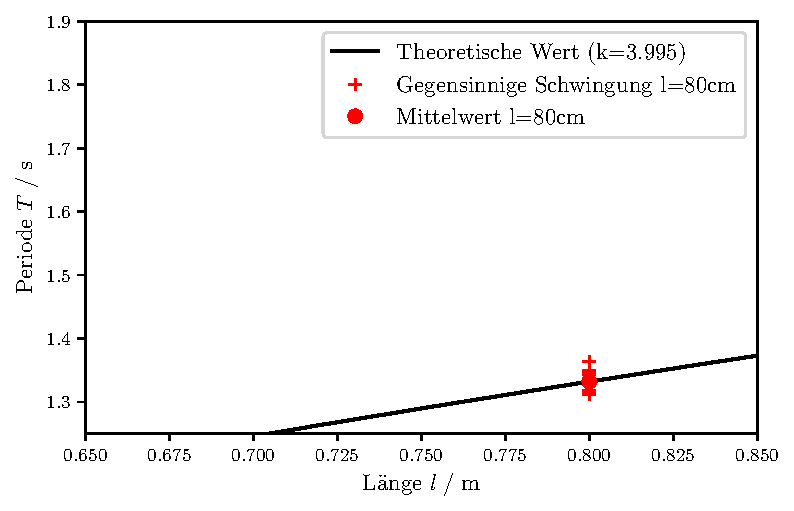
\includegraphics{build/plot5.pdf}
    \caption{Hall Spannung in Abhängigkeit vom Magnetfeld - Kupfer}
    \label{fig:Cu_I}
\end{figure}
Mit der Ausgleichsgeraden
\begin{align*}
    y &= mx + b\\
    m &= \cdot (1,93\pm0,15)10^{-5}\\
    b &=  -0.409006\pm 0.001123\\ % Signifikante Stellen????
\end{align*}

\subsubsection{Bestimmung der mikroskopischen Parameter}
Über die gemessene Hall Spannung,das dazugehörige B-Feld und den Querstrom kann man über \ref{eqn:U_Hall} auf die Anzahl der Ladungsträger pro Volumen schließen.
\begin{equation*}
    
\end{equation*}
% --------SILBER
\subsection{Silber}
\subsubsection{Geometrische Messungen und Wiederstand}
\subsubsection{Hall Spannung bei konstantem B-Feld}
\subsubsection{Hall Spannung bei konstantem Querstrom}
\subsubsection{Bestimmung der mikroskopischen Parameter}
% --------ZINK
\subsection{Zink}
\subsubsection{Geometrische Messungen und Wiederstand}
\subsubsection{Hall Spannung bei konstantem B-Feld}
\subsubsection{Hall Spannung bei konstantem Querstrom}
\subsubsection{Bestimmung der mikroskopischen Parameter}
\label{sec:Auswertung}
